\documentclass{article}

\usepackage[bidi=default]{babel}
\usepackage{amsmath}
\usepackage{amssymb}
\usepackage{algorithm}
\usepackage{algpseudocode}
\usepackage{enumitem}
\usepackage{titlesec}
\usepackage{mathtools}

\DeclarePairedDelimiter\abs{\lvert}{\rvert}
\DeclarePairedDelimiter\norm{\lVert}{\rVert}

\babelprovide[import]{hebrew}
\babelfont{rm}{Frank Ruehl CLM}

\begin{document}
% \selectlanguage{hebrew}
\title{\caption{\foreignlanguage{hebrew}{התמרת רשת משולשים לרשת מרובעים באופן חלק ואינטראקטיבי}}}
\author{וליץ' רועי}
\maketitle

% \selectlanguage{english}
\begin{figure}[ht]
\centering
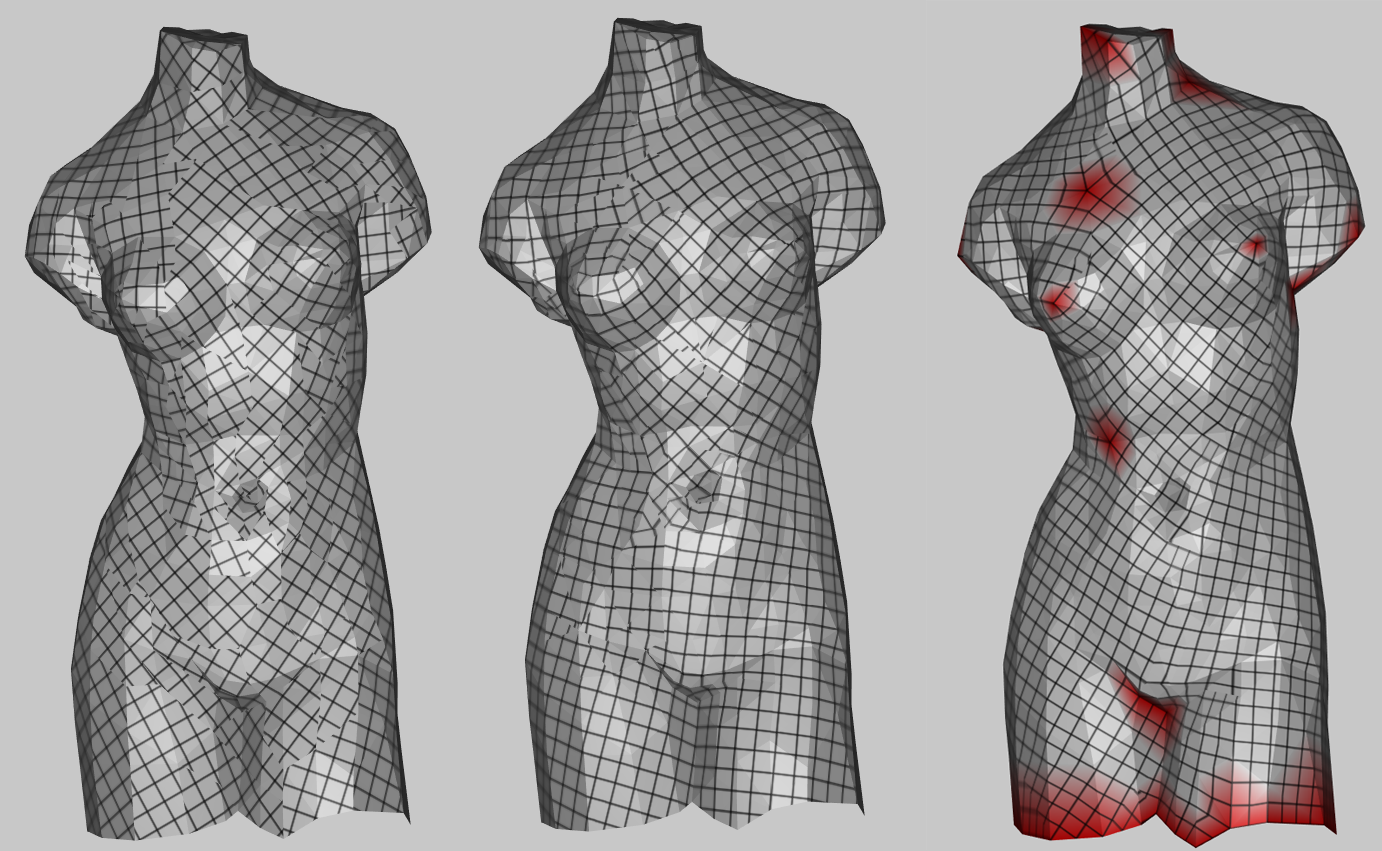
\includegraphics[width=12cm]{teaser.png}
% \selectlanguage{hebrew}
\texthebrew{\caption{\foreignlanguage{hebrew}{
\textbf{שמאל}:
תוצאת העתקת הרשת הקרטזית אל פני המשטח, לאחר המיפוי ההתחלתי של רשת המשולשים למישור
\textbf{מרכז}:
לאחר העלאת המשקולות על פונקציות המחיר
\textbf{ימין}:
התוצאה הסופית המתקבלת לאחר התכנסות תהליך האופטימיזציה למינימום מקומי המקיים את התנאים ההכרחיים והמספיקים להיווצרות רשת מרובעים ע"ג המשטח התלת מימדי
}}}
\label{fig:teaser}
\end{figure}

\selectlanguage{hebrew}
\section{הקדמה}
יישומים רבים בגרפיקה ממוחשבת, לדוגמא עיצוב דמויות ואנימציה, גיאומטריה אדריכלית, וגם סימולציה פיזית במידה מסוימת, דורשים רשת מרובעים 
\foreignlanguage{english}{Quad Mesh}
לייצוג של הגיאומטריה. עם זאת, מכיוון שמודלים מבוססי רשת משולשים
\foreignlanguage{english}{Triangle Mesh}
בדרך כלל נפוצים יותר, יש להמיר אותם באמצעות התהליך המכונה 
\foreignlanguage{english}{Quad Remeshing}.

טכניקות רבות הוצגו בשנים האחרונות, והגישה הנפוצה ביותר היא לפצל את הבעיה לייצור שדה אוריינטציה ע"ג רשת המשולשים בשלב הראשון, ומיפוי המשולשים למישור פרמטריזציה (בהנחיית השדה) בשלב השני. במסמך זה אנו מציגים גישה אינטראקטיבית ישירה וחלקה, שמבטלת את הצורך בשלבי ביניים.
הרעיון העומד מאחורי שיטות מבוססות פרמטריזציה באופן כללי, הוא למפות את רשת המשולשים המקורית למישור, וליצור עליה פריסת רשת קרטזית
\foreignlanguage{english}{Cartesian Grid}
רגילה. על מנת להבטיח שהפריסה הקרטזית במישור הופכת לרשת מרובעת תקפה על פני השטח, יש למלא תנאים מסוימים בפרמטריזציה 
\cite{bommes:hal-00862648},
המפורטים כדלהלן:
\paragraph{\foreignlanguage{english}{Seamless Condition} אי-נראות חתכים}
פונקציית המעבר
$ g_ {ij} $
בין שני חצאי קשתות
$ e_i $
ו-
$ e_j $
במישור הפרמטריזציה, המתאימים לאותה קשת המהווה חלק מחתך ע"ג רשת המשולשים המקורית, יש להיות אוטומורפיזם
\foreignlanguage{english}{Integer Grid Automorphism}
הניתן ע"י:
$$e_j = R^{r_{ij}}_{90^\circ}e_i + \vec{t}_{ij}$$
  כאשר
$r_{ij} \in \{0,1,2,3\}$ and $\vec{t}_{ij} \in \mathbb{Z}^2$.
\paragraph{\foreignlanguage{english}{Singular Points Condition} נקודות סינגולריות}
כל הקודקודים הסינגולריים, המאופיינים בפגם
זוויתי שאינו אפס במישור הפרמטריזציה, חייבים
להיות במיקומים שלמים ע"ג הרשת הקרטזית.
כלומר, בהינתן הקבוצה
$S_i$
של כל הקודקודים בתחום הפרמטריזציה, המתאימים כולם לאותו קודקוד
$v_i$
ע"ג רשת המשולשים המקורית, אנו דורשים כי:
$$\forall u \in S_i: u \in \mathbb{Z}^2 $$
\paragraph{\foreignlanguage{english}{Consistent Orientation Condition} כיוון משולשים עקבי}
כל המשולשים בתחום הפרמטריזציה צריכים להיות בעלי אוריינטציה זהה (עם כיוון-השעון או נגד כיוון-השעון). כלומר, אין לאפשר היפוך משולשים לאחר היווצרות המיפוי הראשוני.

\section{הגישה שלנו}
בהשראת \cite{Poranne:Autocuts:2017}, אנו משתמשים בגישה ישירה לבעיה של התמרת רשת משולשים לרשת מרובעים, על ידי ניסוח ופתרון של בעיית אופטימיזציה חלקה ללא אילוצים. אנו מנסחים פונקציות מחיר חלקות עבור שני התנאים הראשונים שהוזכרו לעיל (אי-נראות חתכים ונקודות סינגולריות), ומוסיפים להן פונקציית מחיר נוספת, אנרגיית דיריכלה סימטרית, המונעת היפוך משולשים ומענישה עיוות משולש.

מכיוון שכל פונקציות המחיר שלנו חלקות, אנו יכולים לבטא באופן אנליטי את הגרדיינטים ומטריצות ההסיאן שלהן, ולהשתמש בשיטת ניוטון כדי לפתור באופן איטרטיבי מיפוי שמגדיר רשת מרובעים תקפה על פני המשטח התלת-ממדי.

הגישה החלקה שלנו מאפשרת להמחיש באופן ויזואלי את כל תהליך האופטימיזציה עבור משתמש הקצה ככלי עיצוב אינטראקטיבי, המאפשר למשתמש להנחות את האלגוריתם לתוצאה הרצויה על ידי שינוי הדרגתי של משקולות העונשין, רזולוציית הרשת, הכוונה של כיוון מרובעים באמצעות מברשת כלי, ועוד. המשתמש מקבל משוב מיידי על כל שינוי שהוחל על הגדרות הבעיה. איור
1 לעיל
ממחיש את שלושת השלבים העיקריים בגישה שלנו. ראשית, משטח התלת מימד נחתך למישור. ואז, משקל פונקציית העונש החלק עלה בהדרגה. לבסוף, פונקציית העונש של נקודות בודדות מופעלת כדי להציב קודקודים בודדים במיקומים שלמים.
\section{אתחול}
אנו חותכים את רשת המשולשים על ידי מיפוי העץ הפורש הדואלי שלה למישור הפרמטריזציה באופן איזומטרי כ-"מרק משולשים"
\foreignlanguage{english}{Triangle Soup}
(פרטים נוספים על מושג זה ניתן למצוא בעבודת התזה המלאה).

ראשית אנו ממפים משולש שרירותי למישור הפרמטריזציה. לאחר מכן אנו ממפים למישור את כל המשולשים הסמוכים לו, אשר חולקים עימו קשת משותפת. אנו ממשיכים בתהליך זה אל עבר השכבה הבאה של משולשים שכנים, עד אשר כל משולשי הרשת ממופים למישור.
\section{
פונקציות מחיר
עבור אי-נראות
חתכים
\foreignlanguage{english}{(Seamless Penalty Functions)}
}
\paragraph{
פונקציית מחיר עבור הפרש זוויתי
\foreignlanguage{english}{(Angle Penalty Function)}
}
בהינתן שני חצאי קשתות
$e_i$
 ו- 
$e_j$ 
בתחום הפרמטריזציה, אנו מגדירים את הפונקציית המחיר עבור ההפרש הזוויתי ביניהן, באופן הבא:
\begin{flalign*}
P_{\mathrm{angle}}\left(e_i,e_j\right) = \sin\left(4\left(\theta(e_i) - \theta(e_j) \right) - \frac{\pi}{2} \right) + 1
\end{flalign*}
כאשר 
$\theta\left(e_i\right)$
 ו- 
$\theta\left(e_j\right)$ 
הם הזווית שיוצרים חצאי הקשתות
$ e_i $
ו- 
$ e_j $ 
עם קו אופקי ע"ג במערכת הצירים הקרטזית, בהתאמה.
נשים לב כי לכל
$k \in \mathbb{Z}$ 
כך ש-
$\theta(e_i) - \theta(e_j) = \frac{\pi}{2}k$
מתקיים כי 
$P_{\mathrm{angle}}\left(e_i,e_j\right) = 0$.
לכן, 
$ P_{\mathrm{angle}}$ 
מענישה חצי קשתות אשר פער הזווית שלהם שונה ממכפלה של
$90^\circ$
\paragraph{
פונקציית מחיר עבור הפרש אורכי צלעות
\foreignlanguage{english}{(Length Penalty Function)}
}
אנו מענישים פערים בהפרש אורכים בין שני חצאי קשתות באמצעות פונקציית המחיר הבאה:
\begin{flalign*}
P_{\mathrm{length}}\left(e_i,e_j\right) = \left( \norm{e_i}^2 - \norm{e_j}^2 \right)^2
\end{flalign*}
יש לשים לב כי רק כששני חצאי הקצוות הם באותו אורך, מתקבל כי
$P_{\mathrm{length}}\left(e_i,e_j\right) = 0$,
ובכל מצב אחר נקבל כי
$P_{\mathrm{length}}\left(e_i,e_j\right) > 0$.
\paragraph{
פונקציית מחיר עבור הזזה שלמה
\foreignlanguage{english}{(Translation Penalty Function)}
}
אנו מענישים שני חצאי קשתות אשר לא משרות הזזה שלמה ביניהן, באופן הבא:
\begin{flalign*}
P_{\mathrm{translation}}\left(e_i,e_j\right) &= \sin\left(2\pi\left(x_{e_i} - x_{e_j}\right) - \frac{\pi}{2} \right) + 1 \\ & \quad + \sin\left(2\pi\left(y_{e_i} - y_{e_j}\right) - \frac{\pi}{2} \right) + 1 \notag
\end{flalign*}
כאשר
$\left(x_{e_i}, y_{e_i}\right)$
ו- 
$\left(x_{e_j}, y_{e_j}\right)$
 הן הקואורדינטות של שני קודקודים תאומים בין שני חצאי הקשתות
$e_i$ 
ו-
$e_j$.
\section{
פונקציית מחיר
עבור נקודות
סינגולריות
\foreignlanguage{english}{(Singular Points Penalty Function)}
}
כדי לעמוד בתנאי הנקודות הסינגולריות, כל הקודקודים התאומים בתחום הפרמטריזציה חייבים להיות על מיקומים שלמים, אם הנקודה המתאימה להם ע"ג המשטח התלת-מימדי היא נקודה סינגולרית. לכן אנו מענישים קודקודים-תאומים של נקודות סינגולריות באופן הבא:
\begin{flalign*}
P_{\mathrm{singular}}\left(S\right) = \sum_{v \in S} \left( \sin\left(2 \pi x_{v} - \frac{\pi}{2} \right) + 1 + \sin\left(2 \pi y_{v} - \frac{\pi}{2} \right) + 1 \right)
\end{flalign*}
כאשר
$S$
היא קבוצה של קודקודים תאומים בתחום הפרמטריזציה המתאימים לנקודה סינגולרית ע"פ המשטח, ו- 
$\left(x_v,y_v\right)$
 הן הקואורדינטות של קודקוד התחום
$v \in S$.
\section{
פונקציית מחיר עבור עיוות וכיוון-עקבי של משולשים
\foreignlanguage{english}{(Consistent Orientation and Distortion Penalty Function)}
}
כדי לספק את תנאי האוריינטציה העקבית של משולשים, וכדי למזער עיוות משולשים, אנו משתמשים באנרגיית דיריכלה סימטרית
\cite{Smith:2015}
המונעת היפוך משולשים ומקדמת מיפויים איזומטריים. פונקציית מחיר עבור אנרגיית דיריכלה סימטרית ניתנת כדלקמן:
\begin{flalign*}
P_{\mathrm{dirichlet}}\left(t_i\right) = \norm{J\left(t_i\right)}_F^2 + \norm{J^{-1}\left(t_i\right)}_F^2
\end{flalign*}
כאשר
$J\left(t_i\right)$
הוא היעקוביאן של מיפוי המשולש 
$t_i$
ו- 
$\norm{\cdot}_F$
היא נורמת פרובניוס של מטריצות.

\section{
אופטימיזציה
\foreignlanguage{english}{(Optimization Process)}
}
על מנת למצוא פרמטריזציה המהווה רשת-מרובעים תקפה על פני השטח התלת-ממדי, אנו פותרים את בעיית האופטימיזציה ללא-אילוצים הבאה:
\begin{flalign*}
\min_{X} & \quad \sum_{i \sim j} \Big( P_{\mathrm{angle}}\left(e_i,e_j\right) + P_{\mathrm{length}}\left(e_i,e_j\right) + P_{\mathrm{translation}}\left(e_i,e_j\right) \Big) \\
 & + \sum_{i} P_{\mathrm{singular}}\left(S_i\right) \notag \\
 & + \sum_{i} P_{\mathrm{dirichlet}}\left(t_i\right) \notag
\end{flalign*}
כאשר
$X$
מציין את קבוצת המשתנים של בעיית האופטימיזציה, כלומר את הקואורדינטות של הקודקודים בתחום הפרמטריזציה. אנו מפתחים ביטויים אנליטיים לגראדיינט ולהסיאן של כל פונקציית מחיר, ועורכים את ההסיאנים המחושבים, במידת הצורך, כך שהם יהיו מוגדרים-חיובית (על ידי שימוש בפירוק
SVD
ואיפוס ערכים סינגולרים שליליים). אנו פותרים את בעיית האופטימיזציה בשיטת ניוטון. באיטרציה 
$i$
אנו מעריכים את הגראדיינט
$g^{(i)}$
וההסיאן 
$H^{(i)}$
של הפונקציה המטרה הכוללת שלנו ב- 
$X^{(i)}$
ופותרים את מערכת המשוואות הלינארית הדלילה 
$H^{(i)}d^{(i)}=-g^{(i)}$
שמניבה כיוון חיפוש
$d^{(n)}$
האיטרציה הבאה מתקבלת על ידי
$X^{(i+1)} = X^{(i)} + \alpha p^{(i)}$
כאשר ה- 
$\alpha$
האופטימלי נמצא באמצעות אלגוריתם
Line Search.
אנו משתמשים בחבילת התוכנה
\foreignlanguage{english}{MKL PARDISO}
של אינטל בכדי לפתור את מערכת המשוואות הליניאריות הדלילה המושרות על ידי שיטת ניוטון.
\section{תוצאות}
לסוף המסמך מצורפות תוצאות הרצה של כלי המממש את השיטה את השיטה שתיארנו לעיל, על שלושה מודלים שונים של רשתות-משולשים.
\newpage
\selectlanguage{english}
\begin{figure}[ht]
\centering
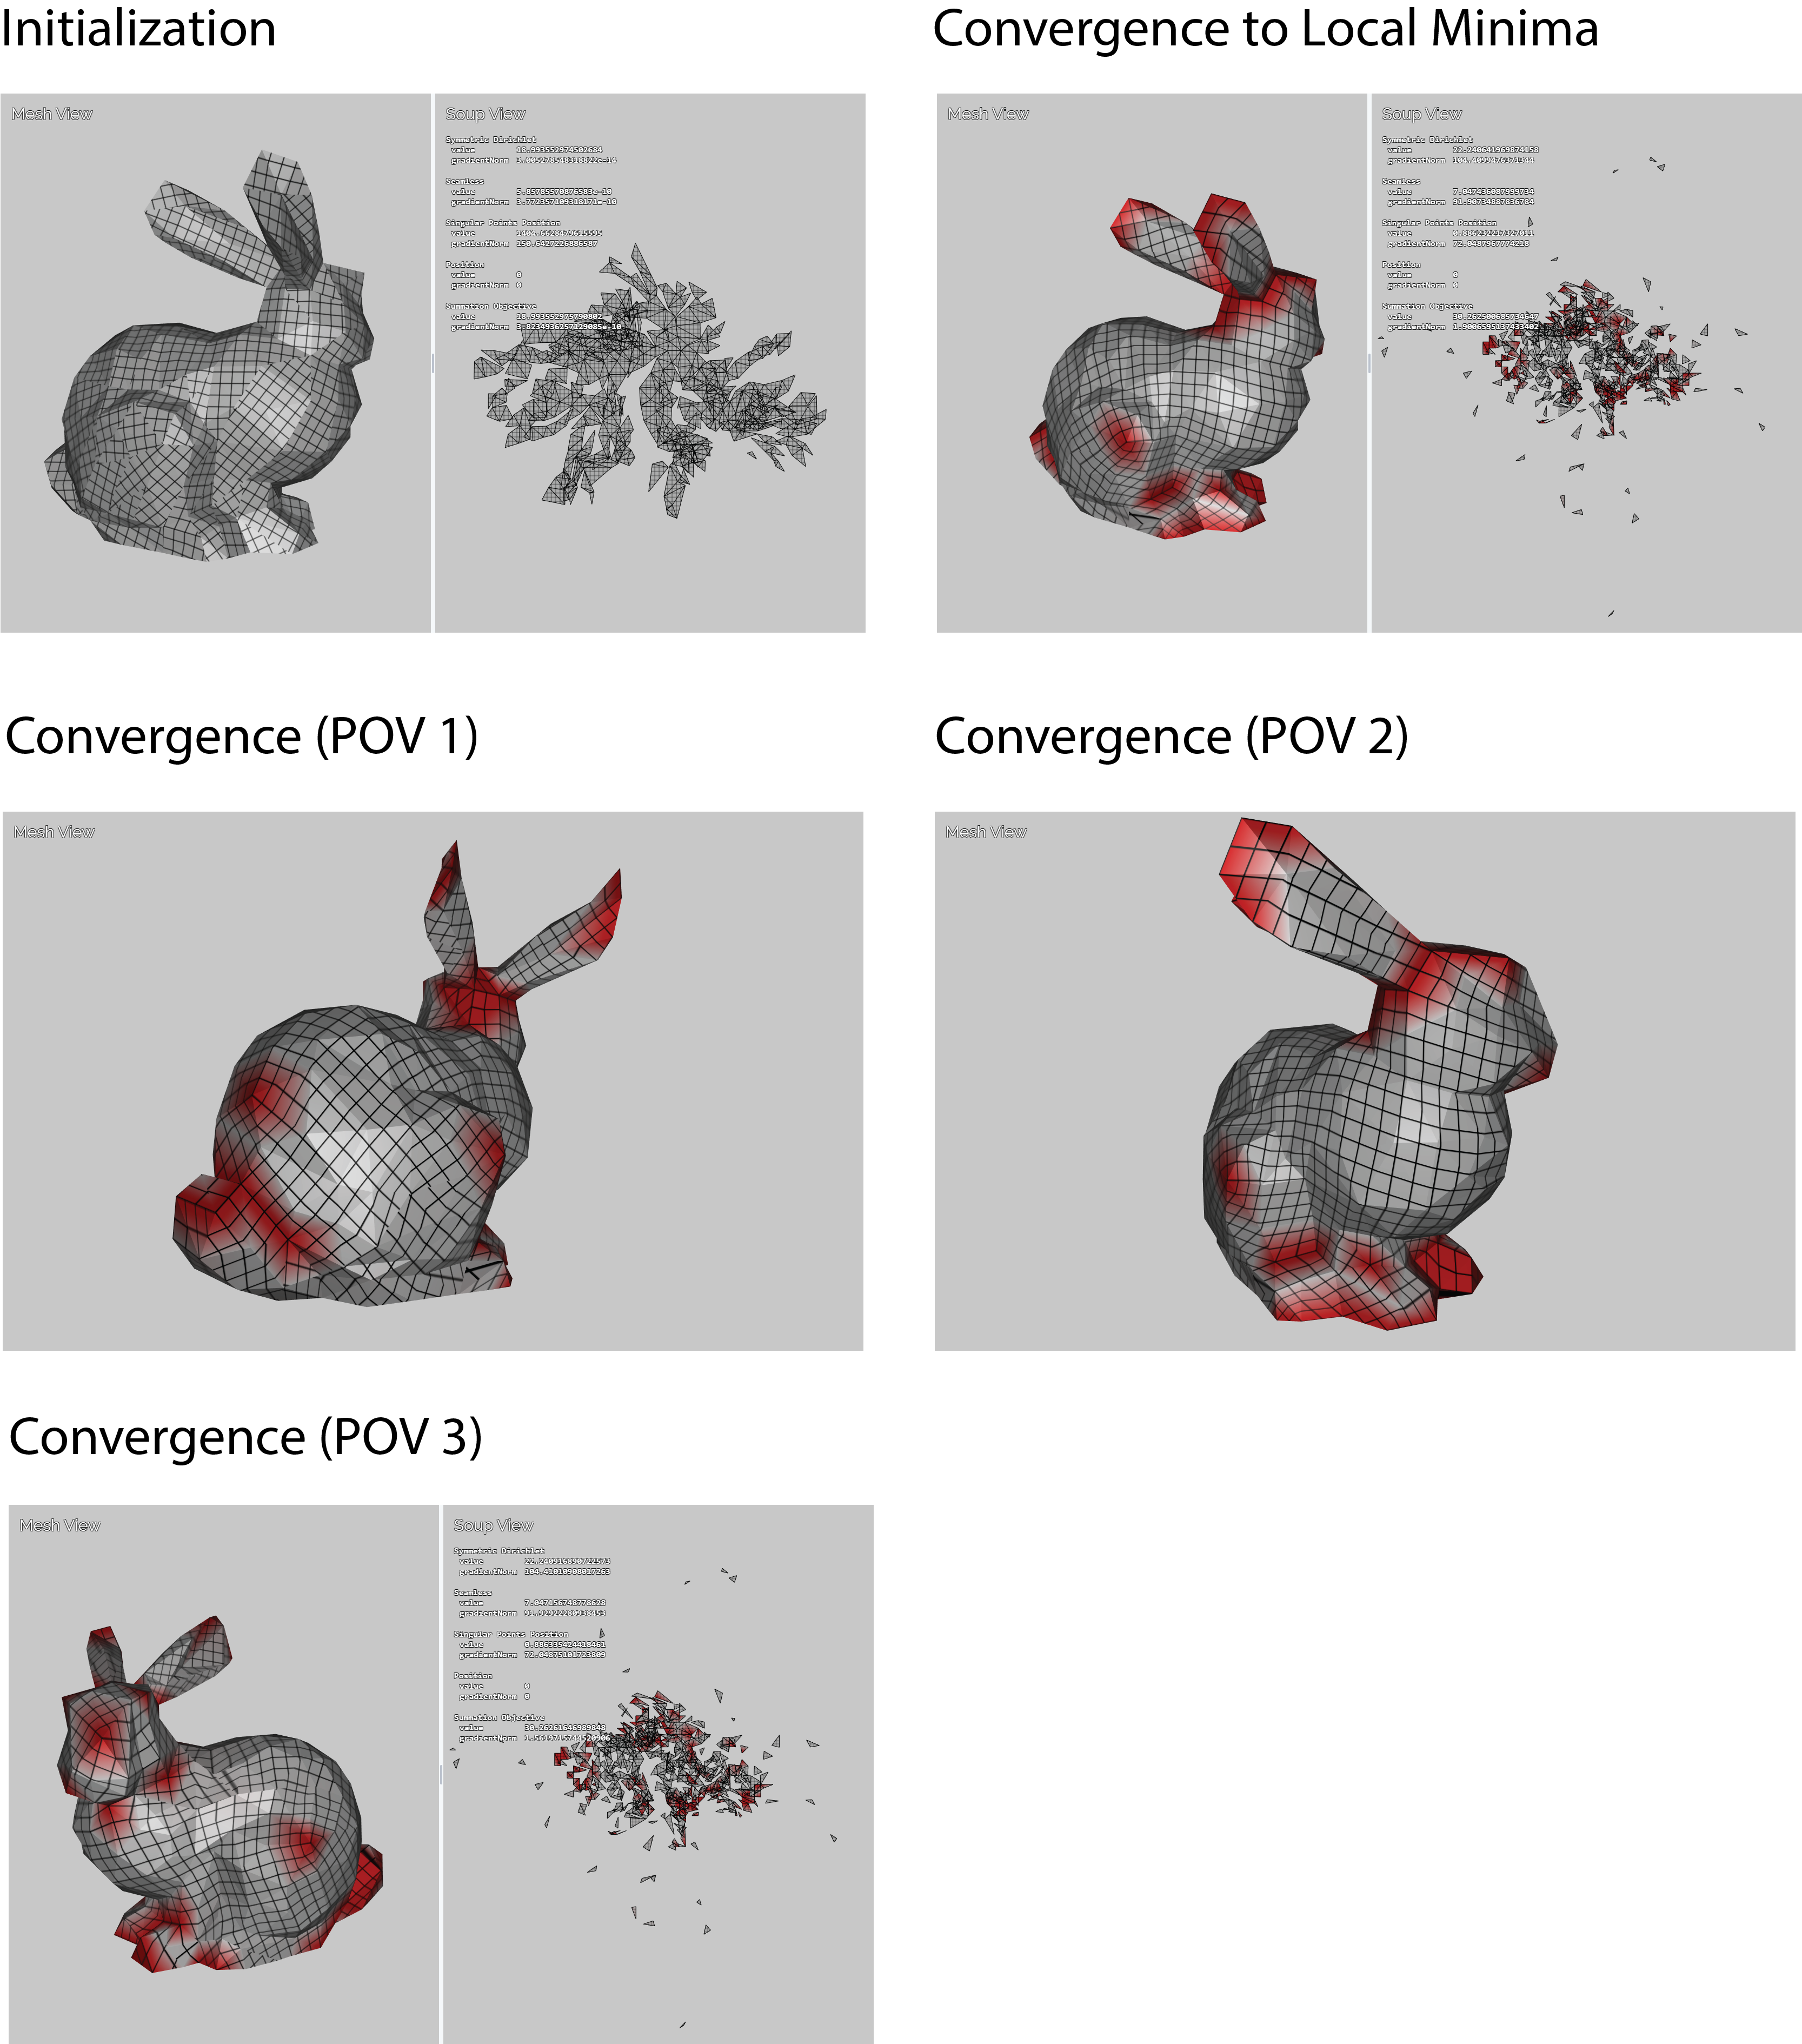
\includegraphics[width=14cm]{bunny.png}
\end{figure}
\newpage
\selectlanguage{english}
\begin{figure}[ht]
\centering
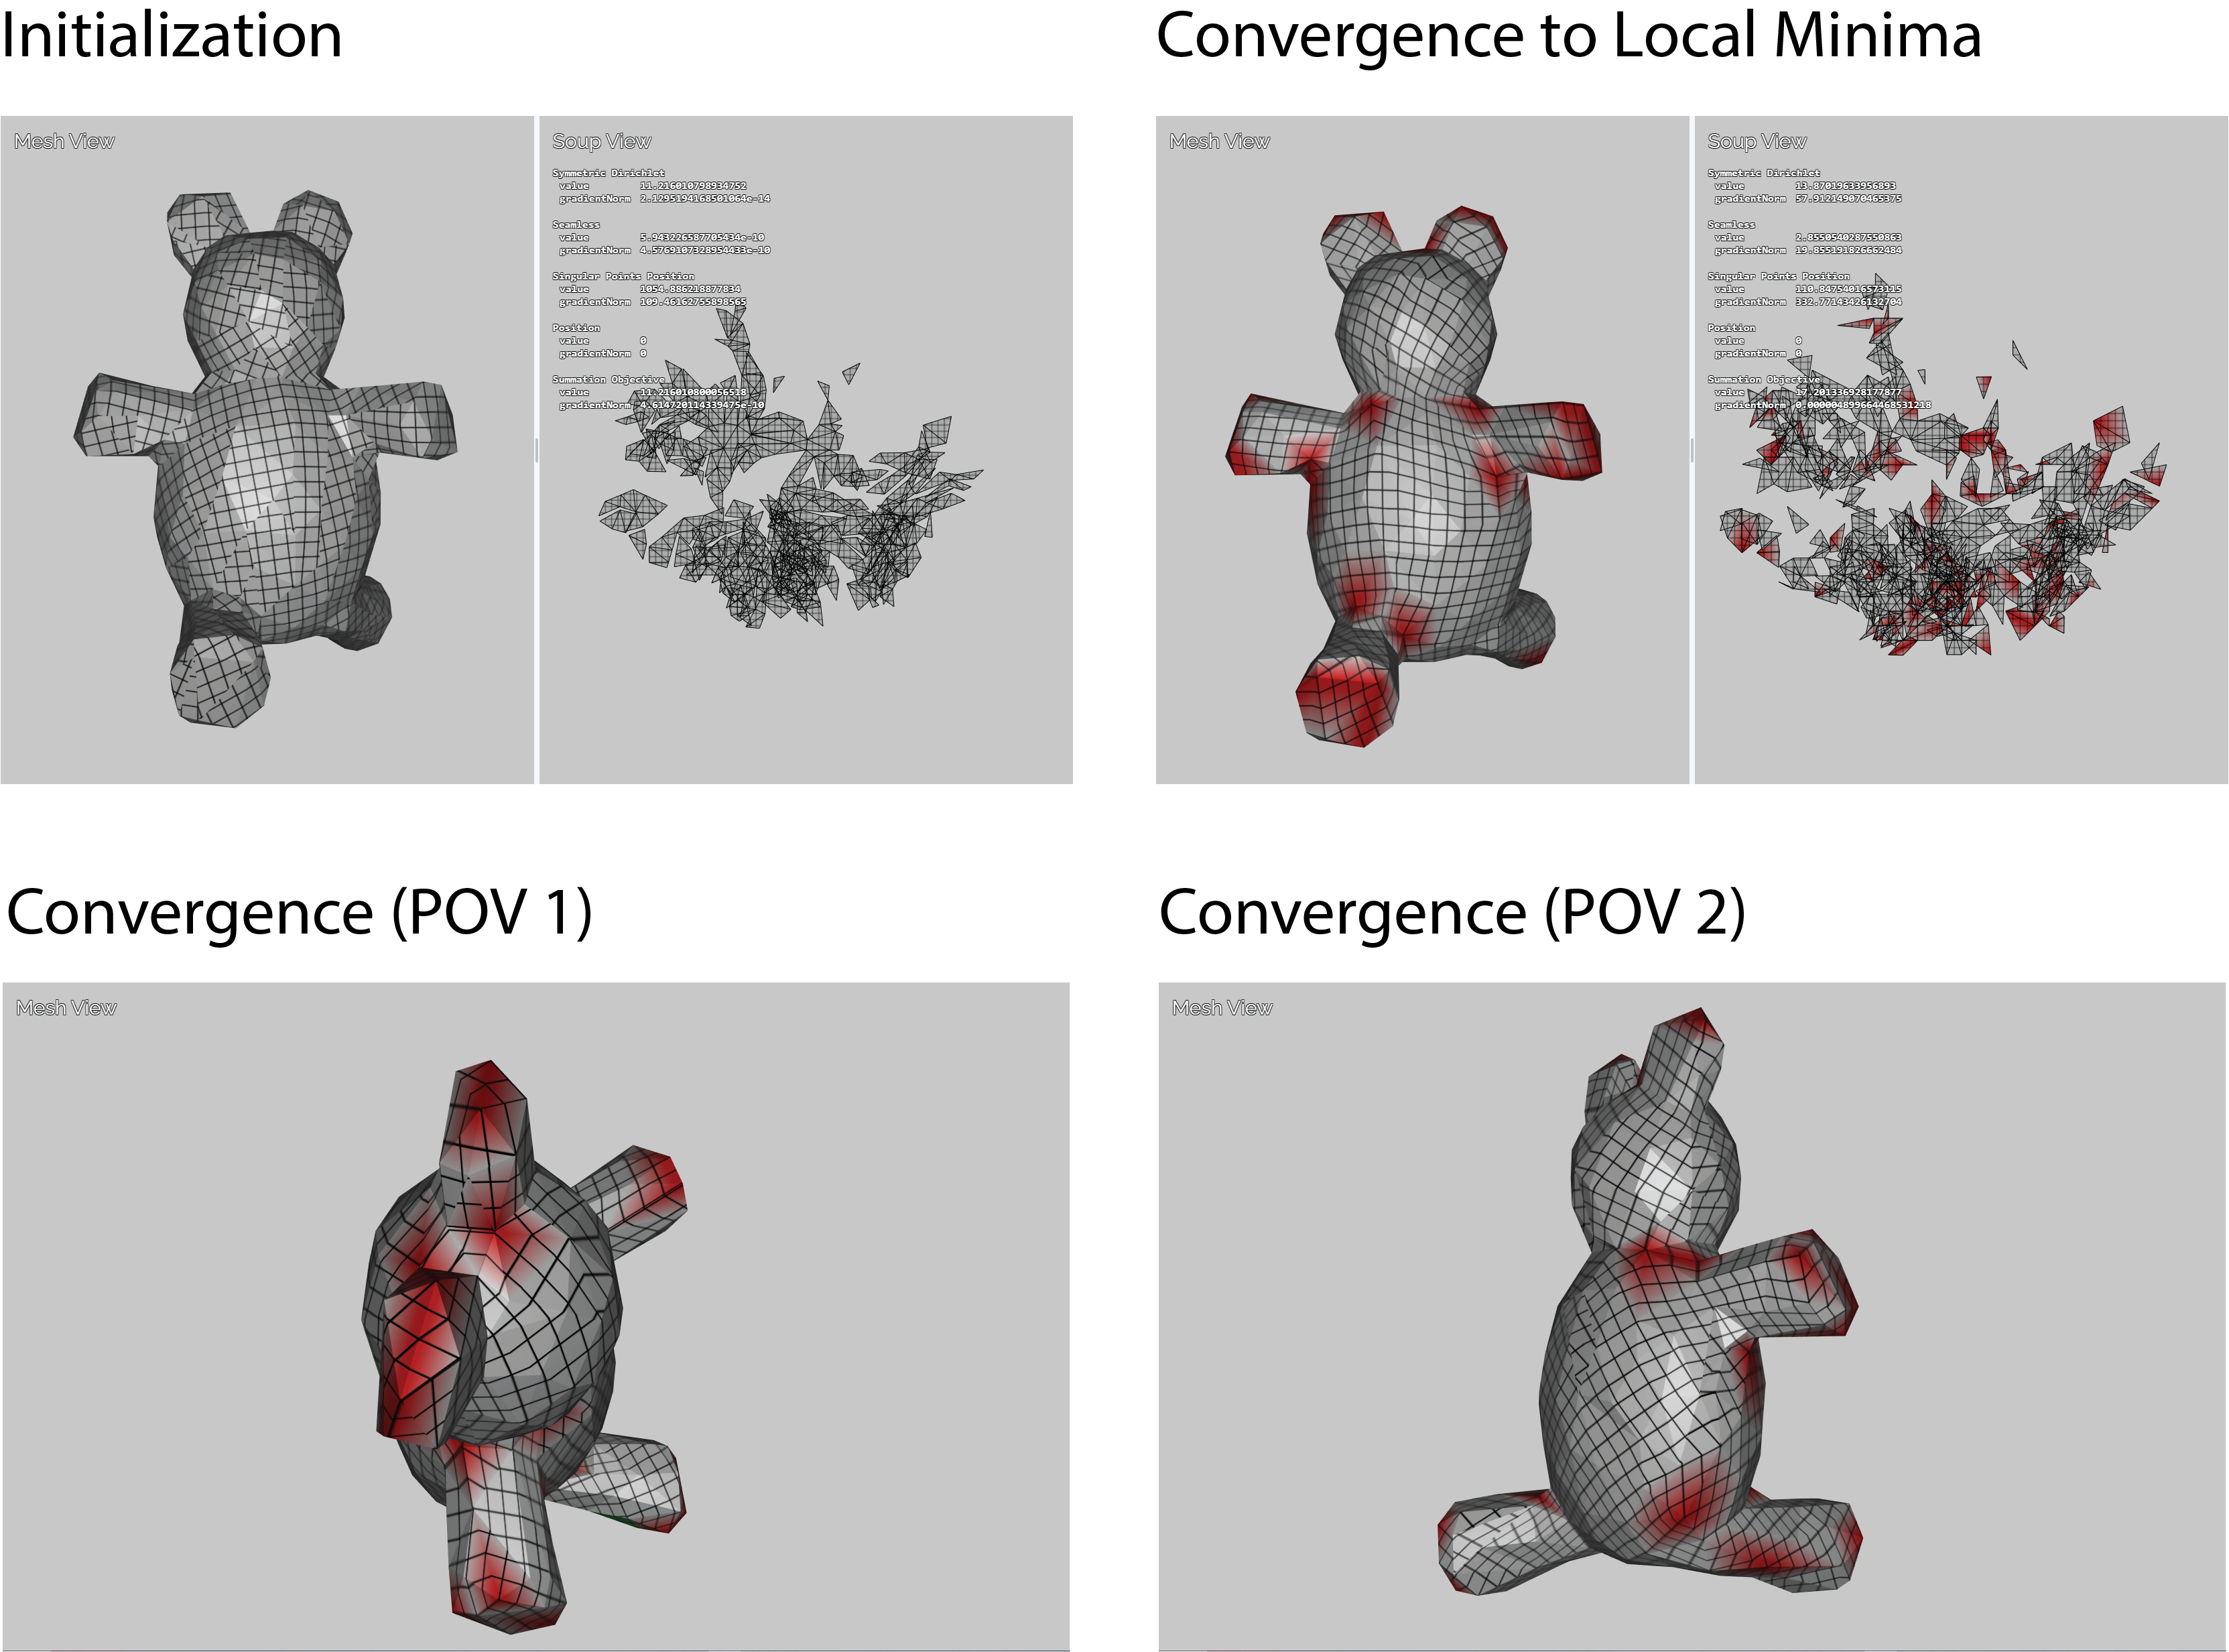
\includegraphics[width=14cm]{teddy.png}
\end{figure}
\newpage
\selectlanguage{english}
\begin{figure}[ht]
\centering
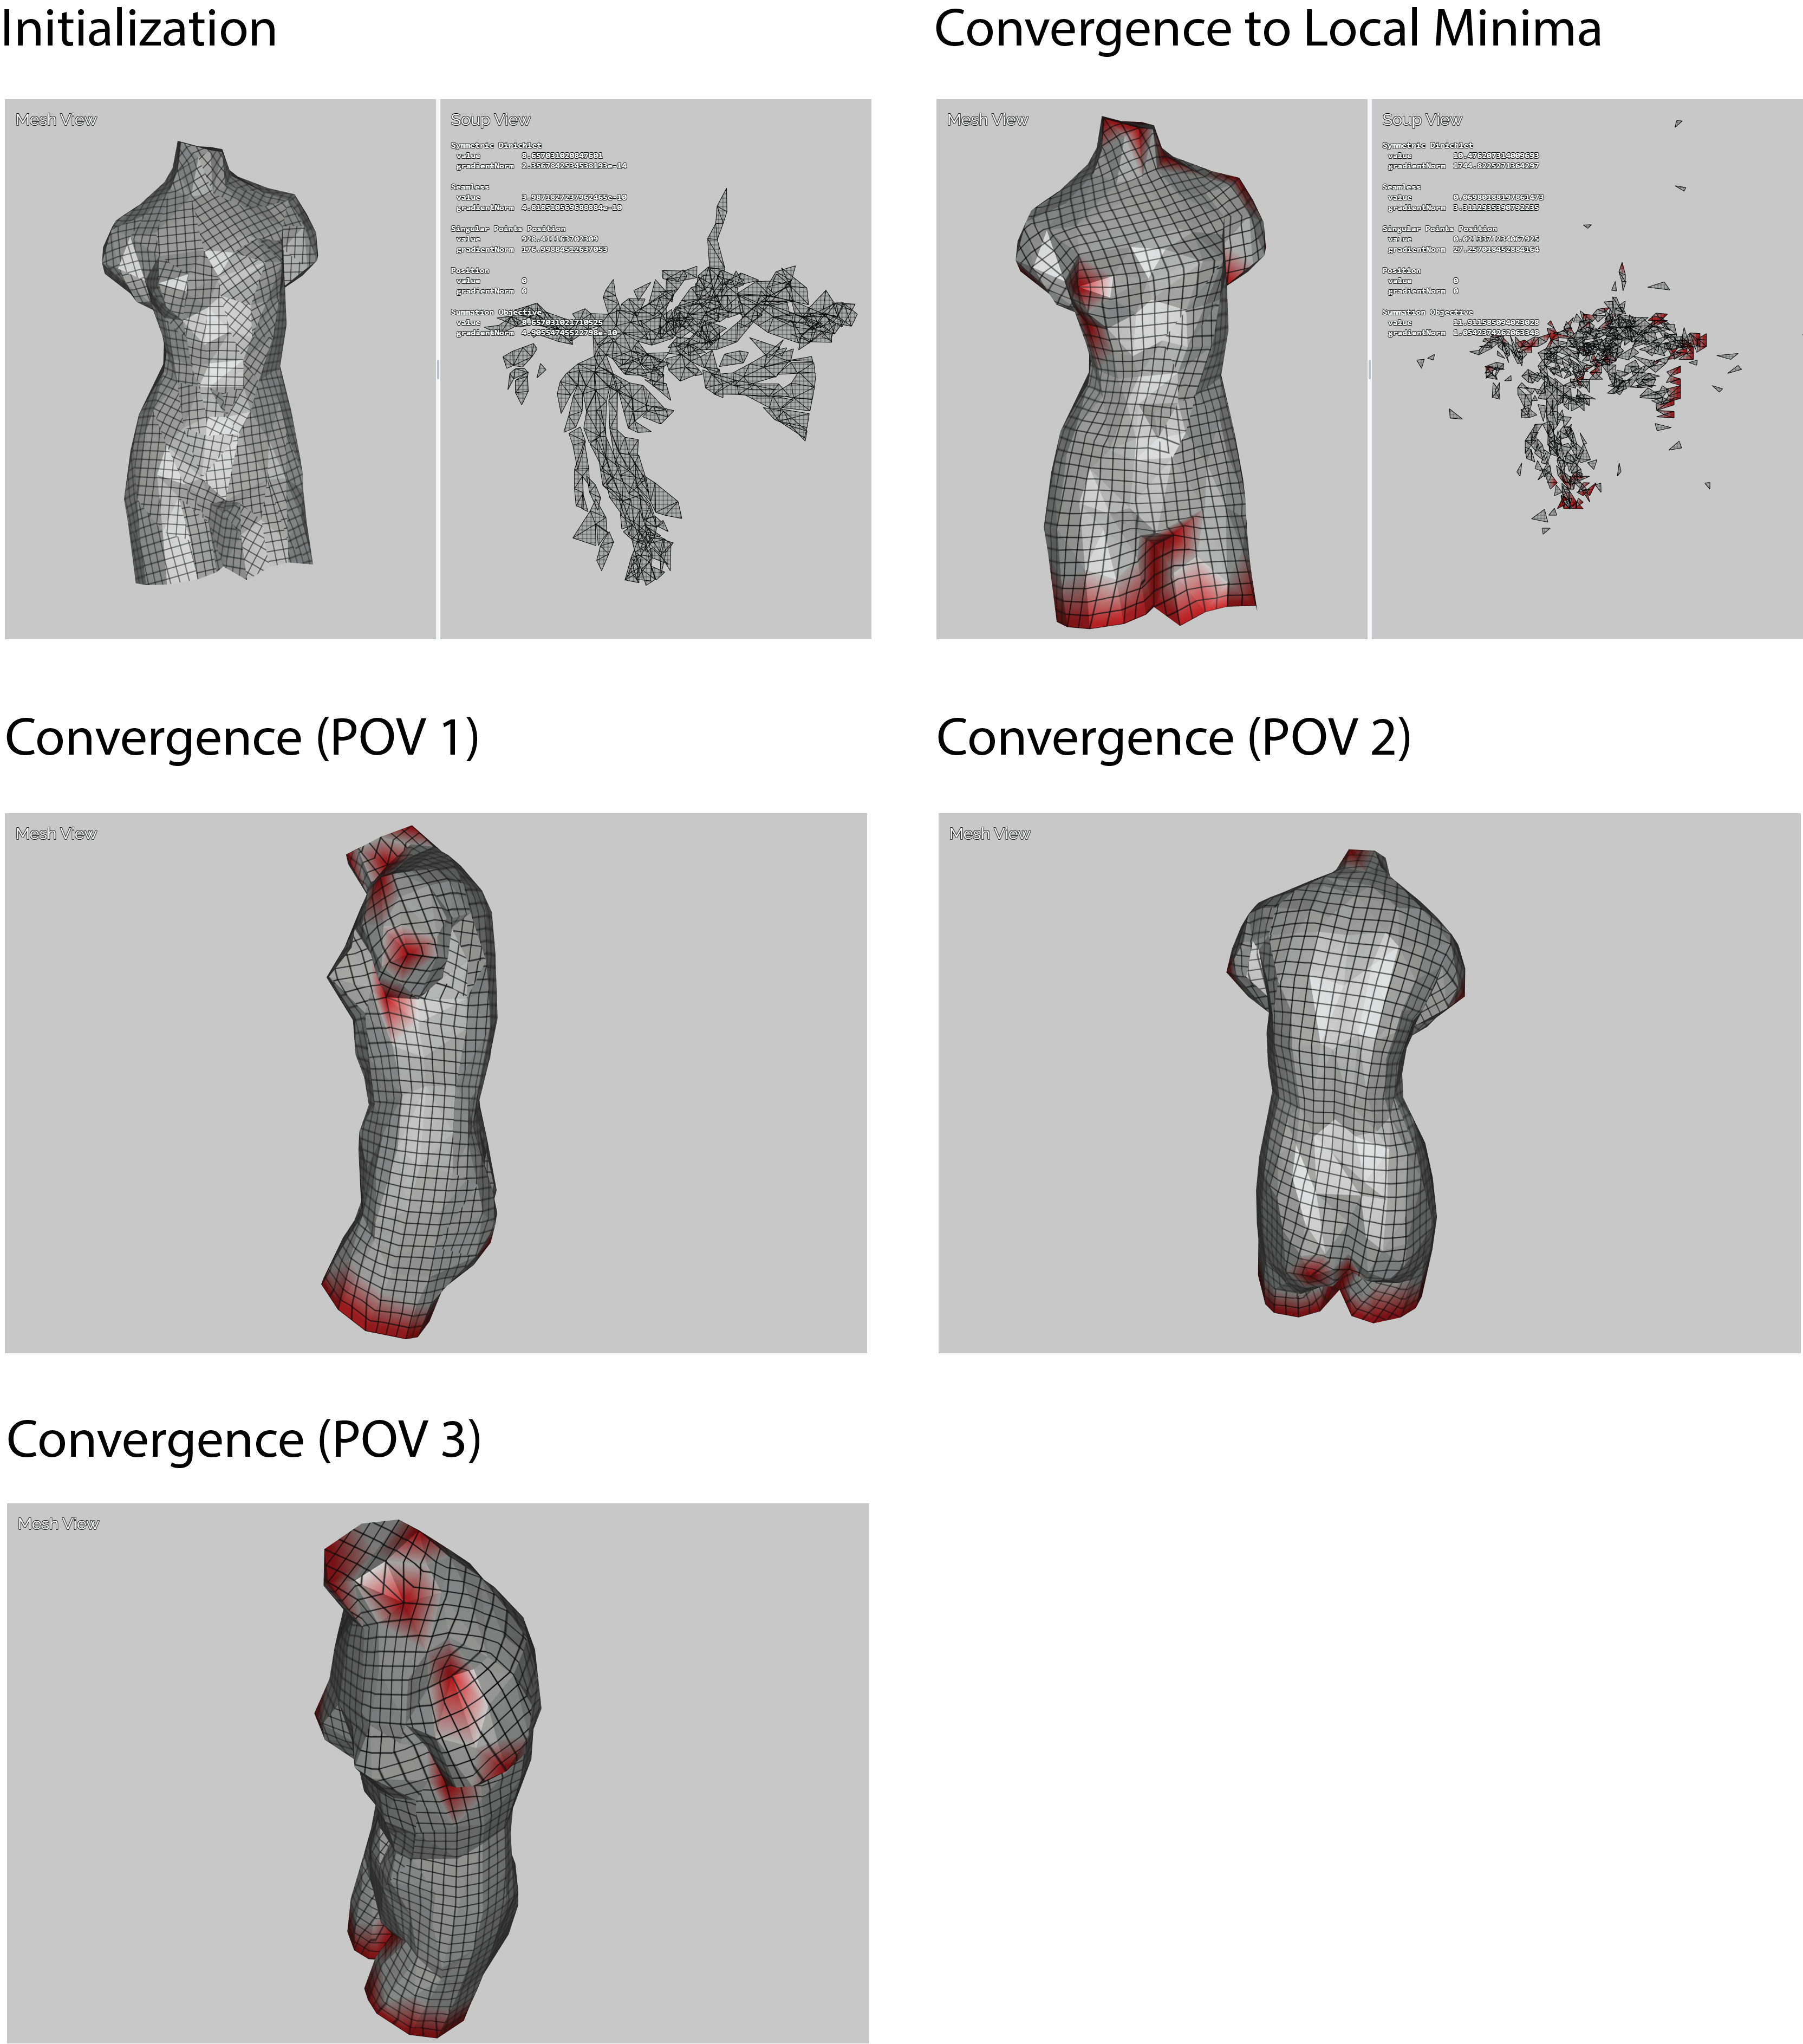
\includegraphics[width=14cm]{venus.png}
\end{figure}
\selectlanguage{hebrew}
\bibliographystyle{unsrt}
\bibliography{main}
\end{document}
